\documentclass{sjtuarticle}
\allowdisplaybreaks[1]
\usepackage{array}
\usepackage{ntheorem}
\usepackage{float}
\usepackage{pgfplots}
\pgfplotsset{compat=newest}
\usepackage{bm}
\usepackage{booktabs}
\usepackage{subcaption}
\usepackage[colorlinks]{hyperref}

\def\dd{\mathrm{d}}

\title{作业6}
\author{Log Creative}
\date{2023 年 12 月 8 日}
\begin{document}
\maketitle

% P78:3,9,14 ,16,17,22,其中22题修改见附件

\begin{itemize}
    \item[3.] \begin{solution}
        对于 $f(x)=\sin 4x$ 于 $[0,2\pi]$ 而言,对于 $P(x)=0$,有 Chebyshev 交错点组 $\frac{\pi}{8}$,$\frac{3\pi}{8}$,$\frac{5\pi}{8}$,$\frac{7\pi}{8}$,$\frac{9\pi}{8}$,$\frac{11\pi}{8}$,$\frac{13\pi}{8}$,$\frac{15\pi}{8}$ 共 8 个点,则 $P(x)=0$ 是 $f(x)=\sin 4x$ 在 $[0,2\pi]$ 上的最佳一致逼近多项式,由于 $f(x)\in C[0,2\pi]$,所以它是唯一的。
        
        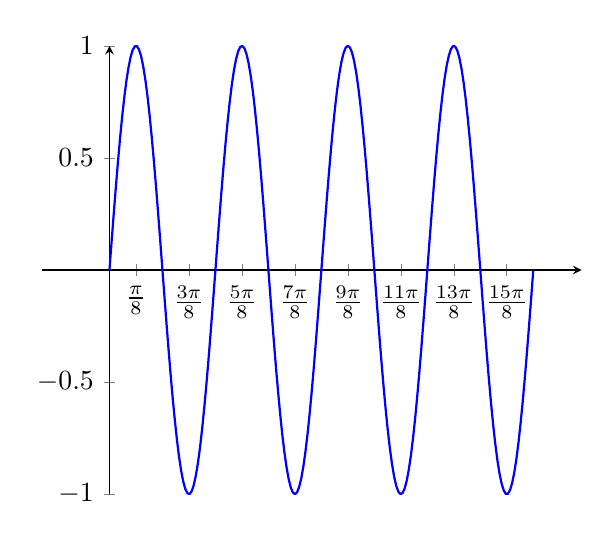
\begin{tikzpicture}
            \begin{axis}[axis x line={middle},
            axis y line={middle},
            xmax={7},
            xmin={-1},
            xlabel={},
            ylabel={},
            xtick={0.393,1.178,1.963,2.749,3.534,4.320,5.105,5.890},xticklabels={$\frac{\pi}{8}$,$\frac{3\pi}{8}$,$\frac{5\pi}{8}$,$\frac{7\pi}{8}$,$\frac{9\pi}{8}$,$\frac{11\pi}{8}$,$\frac{13\pi}{8}$,$\frac{15\pi}{8}$},]
            \addplot [domain=0:6.282,samples=202,thick,blue,] {sin(4*deg(x))};
            \end{axis}
        \end{tikzpicture}
    \end{solution}
    \item[9.] \begin{solution}
        令 $t=2x-1$,则变量代换后,
        \begin{equation*}
            g(t)=\left(\frac{t+1}{2}\right)^4+3\left(\frac{t+1}{2}\right)^3-1=\frac{t^{4}}{16} + \frac{5 t^{3}}{8} + \frac{3 t^{2}}{2} + \frac{11 t}{8} - \frac{9}{16}
        \end{equation*}
        根据 Chebyshev 多项式定理,当
        \begin{equation*}
            g(t)-Q^*_3(t)=\frac{1}{16}\cdot\frac{1}{2^3}T_4(t)=\frac{1}{2^7}(8t^4-8t^2+1)
        \end{equation*}
        时,与零偏差最小,故
        \begin{equation*}
            % latex(expand('((x+1)/2)**4+3*((x+1)/2)**3-1-1/(2**7)*(8*x**4-8*x**2+1)'))
            Q^*_3(t)=\frac{5 t^{3}}{8} + \frac{25 t^{2}}{16} + \frac{11 t}{8} - \frac{73}{128}
        \end{equation*}
        将 $t=2x-1$ 代回,有
        \begin{equation*}
            % latex(expand(expand('((x+1)/2)**4+3*((x+1)/2)**3-1-1/(2**7)*(8*x**4-8*x**2+1)').subs(x,2*x-1)))
            P^*_3(x)=5 x^{3} - \frac{5 x^{2}}{4} + \frac{x}{4} - \frac{129}{128}
        \end{equation*}
        为 $f(x)=x^4+3x^3-1$ 的最佳三次逼近多项式。
    \end{solution}
    \item[14.] \begin{solution}
        \begin{itemize}
            \item[(1)] $(f,g)=\int_a^b f^\prime(x)g^\prime(x)\dd x$ 不是内积,因为对于 $(f,f)\geq 0$,当 $f^\prime(x)=c$, $c$ 是常数时,等号依然满足。
            \item[(2)] $(f,g)=\int_a^b f^\prime(x)g^\prime(x)\dd x+f(a)g(a)$ 是内积,验证如下:
            \begin{itemize}
            \item[a.] $(f,g)=(g,f)$:
                \begin{equation*}
                    (f,g)=\int_a^b f^\prime(x)g^\prime(x)\dd x + f(a)g(a)=\int_a^b g^\prime(x)f^\prime(x)\dd x + g(a)f(a)=(g,f)
                \end{equation*}
                \item[b.] $(cf,g)=c(f,g)$,$c$ 是常数:
                \begin{equation*}
                    \begin{aligned}
                        (cf,g)&=\int_a^b (cf)^\prime(x)g^\prime(x)\dd x + cf(a)g(a)\\
                        &=\int_a^b cf^\prime(x)g^\prime(x)\dd x+cf(a)g(a)\\
                        &=c\left(\int_a^b f^\prime(x)g^\prime(x)\dd x+f(a)g(a)\right)\\
                        &=c(f,g)
                    \end{aligned}
                \end{equation*}
                \item[c.] $(f_1+f_2,g)=(f_1,g)+(f_2,g)$:
                \begin{equation*}
                    \begin{aligned}
                        (f_1+f_2,g)&=\int_a^b (f_1(x)+f_2(x))^\prime g^\prime(x)\dd x+(f_1(a)+f_2(a))g(a)\\
                        &=\int_a^b (f_1^\prime(x)+f_2^\prime(x))g^\prime(x)\dd x+(f_1(a)+f_2(a))g(a)\\
                        &=\int_a^b f_1^\prime(x)g^\prime(x)\dd x+f_1(a)g(a)+\int_a^b f_2^\prime(x)g^\prime(x)\dd x+f_2(a)g(a)\\
                        &=(f_1,g)+(f_2,g)
                    \end{aligned}
                \end{equation*}
                \item[d.] $(f,f)\geq 0$,当且仅当 $f=0$ 时 $(f,f)=0$:
                \begin{equation*}
                    (f,f)=\int_a^b f^\prime(x)f^\prime(x)\dd x+f(a)f(a)=\int_a^b (f^\prime(x))^2\dd x+(f(a))^2\geq 0
                \end{equation*}
            \end{itemize}
        \end{itemize}
    \end{solution}
    \item[16.] \begin{solution}
        \begin{itemize}
            \item[(1)]\begin{equation*}
                \int_{-1}^1 (x-ax^2)^2\dd x = \int_{-1}^1 (a^2x^4-2ax^3+x^2) \dd x=\frac{2}{5}a^2+\frac{2}{3}
            \end{equation*}
            $a=0$ 时取得最小值 $\frac{2}{3}$。
            \item[(2)] 当 $a=0$ 时,
            \begin{equation*}
                \int_{-1}^1 |x-ax^2|\dd x = \int_{-1}^1 |x|\dd x = 2\int_0^1 x\dd x=1
            \end{equation*}
            当 $0<a\leq 1$ 时,
            \begin{equation*}
                \int_{-1}^1 |x(1-ax)|\dd x = \int_{-1}^0 (ax^2-x)\dd x + \int_{0}^1 (x-ax^2)\dd x=\frac{1}{3}a+\frac{1}{2}+\frac{1}{2}-\frac{1}{3}a=1 %\left.\left(\frac{1}{3}ax^3-\frac{1}{2}x^2\right)\right|_{-1}^0
            \end{equation*}
            当 $a>1$ 时,
            \begin{align*}
                \int_{-1}^1 |x(1-ax)|\dd x &= \int_{-1}^0 (ax^2-x)\dd x + \int_{0}^\frac{1}{a} (x-ax^2)\dd x + \int_{\frac{1}{a}}^1 (ax^2-x)\dd x\\
                &=\frac{1}{3}a+\frac{1}{2}+\frac{1}{2a^2}-\frac{1}{3a^2}+\frac{1}{3}a-\frac{1}{2}-\frac{1}{3a^2}+\frac{1}{2a^2}\\
                &=\frac{2a}{3}+\frac{1}{3a^2}=\frac{a}{3}+\frac{a}{3}+\frac{1}{3a^2}> 1
            \end{align*}
            等号成立当且仅当 $\frac{a}{3}=\frac{1}{3a^2}$,即 $a=1$,不在范围,所以等号取不到。

            根据对称性可以知道,当 $-1\leq a<0$ 时,$\int_{-1}^1 |x-ax^2|\dd x=1$;当 $a<-1$ 时,$\int_{-1}^1 |x-ax^2|\dd x>1$。

            所以最小值是 1,最小值取在 $|a|\geq 1$。
        \end{itemize}
    \end{solution}
    \item[17.] \begin{solution}
        % 问题等价于寻找 $\Phi=\text{span}\{\phi_0=1,\phi_1=x,\phi_2=x^{100},\phi_3=x^{101}\}$ 上对于 $f(x)=x^2\in C[0,1]$ 的最佳平方逼近,令这个函数为
        % \begin{equation*}
        %     g(x)=\sum_{i=0}^3 a_i \phi_i(x)
        % \end{equation*}
        % 则考察法方程
        % \begin{equation*}
        %     \begin{pmatrix}
        %         (\phi_0,\phi_0) & (\phi_0,\phi_1) & (\phi_0,\phi_2) & (\phi_0,\phi_3) \\
        %         (\phi_1,\phi_0) & (\phi_1,\phi_1) & (\phi_1,\phi_2) & (\phi_1,\phi_3) \\
        %         (\phi_2,\phi_0) & (\phi_2,\phi_1) & (\phi_2,\phi_2) & (\phi_2,\phi_3) \\
        %         (\phi_3,\phi_0) & (\phi_3,\phi_1) & (\phi_3,\phi_2) & (\phi_3,\phi_3)
        %     \end{pmatrix}\begin{pmatrix}
        %         a_0 \\ a_1 \\ a_2 \\ a_3
        %     \end{pmatrix}=\begin{pmatrix}
        %         (f,\phi_0) \\ (f,\phi_1) \\ (f,\phi_2) \\ (f,\phi_3)
        %     \end{pmatrix}
        % \end{equation*}
        % 即
        % \begin{equation*}
        %     \begin{pmatrix}
        %         1 & \frac{1}{2} & \frac{1}{101} & \frac{1}{102} \\
        %         \frac{1}{2} & \frac{1}{3} & \frac{1}{102} & \frac{1}{103} \\
        %         \frac{1}{101} & \frac{1}{102} & \frac{1}{201} & \frac{1}{202} \\
        %         \frac{1}{102} & \frac{1}{103} & \frac{1}{202} & \frac{1}{203}
        %     \end{pmatrix}\begin{pmatrix}
        %         a_0 \\ a_1 \\ a_2 \\ a_3
        %     \end{pmatrix}=\begin{pmatrix}
        %         \frac{1}{3} \\ \frac{1}{4} \\ \frac{1}{103} \\ \frac{1}{104}
        %     \end{pmatrix}
        % \end{equation*}
        % 解得
        % \begin{equation*}
        %     \begin{pmatrix}
        %         a_0 \\ a_1 \\ a_2 \\ a_3
        %     \end{pmatrix}=\begin{pmatrix}
        %         -0.1540 \\ 0.9612 \\ 65.0799 \\ -65.0381
        %     \end{pmatrix}
        % \end{equation*}
        % 故选取 
        \begin{itemize}
            \item[(1)] 对于 $\phi_1=\text{span}\{1,x\}$,考虑法方程
            \begin{equation*}
                \begin{pmatrix}
                    1 & \frac{1}{2} \\ \frac{1}{2} & \frac{1}{3}
                \end{pmatrix}\begin{pmatrix}
                    a_0 \\ a_1
                \end{pmatrix}=\begin{pmatrix}
                    \frac{1}{3} \\ \frac{1}{4}
                \end{pmatrix}
            \end{equation*}
            解得
            \begin{equation*}
                a_0 = -\frac{1}{6}, \quad a_1 = 1
            \end{equation*}
            得到最佳平方逼近函数 $g_1(x)=-\frac{1}{6}+x$。误差为
            \begin{equation*}
                \lVert g_1(x)-f(x) \rVert_2=\sqrt{\int_{0}^1 (g_1(x)-f(x))^2 \dd x}=\sqrt{\int_{0}^1 \left(-\frac{1}{6}+x-x^2\right)^2 \dd x}=0.0745
            \end{equation*}
            \item[(2)] 对于 $\phi_2=\text{span}\{x^{100},x^{101}\}$,考虑法方程
            \begin{equation*}
                \begin{pmatrix}
                    \frac{1}{201} & \frac{1}{202} \\ \frac{1}{202} & \frac{1}{203}
                \end{pmatrix}\begin{pmatrix}
                    a_0 \\ a_1
                \end{pmatrix}=\begin{pmatrix}
                    \frac{1}{103} \\ \frac{1}{104}
                \end{pmatrix}
            \end{equation*}
            解得
            \begin{equation*}
                \begin{pmatrix}
                    a_0 \\ a_1
                \end{pmatrix}=
                \left(\begin{array}{c}
                    \frac{2009799}{5356}\\
                    -\frac{1004647}{2678}
                    \end{array}\right)=\begin{pmatrix}
                        375.2425 \\ -375.1482
                    \end{pmatrix}
            \end{equation*}
            得到最佳平方逼近函数 $g_2(x)=375.2425x^{100}-375.1482x^{101}$。误差为
            \begin{equation*}
                \lVert g_2(x)-f(x) \rVert_2=\sqrt{\int_{0}^1 (g_2(x)-f(x))^2 \dd x}=\sqrt{\int_{0}^1 \left(375.2425x^{100}-375.1482x^{101}-x^2\right)^2 \dd x}=0.4050
            \end{equation*}
        \end{itemize}
        可见前者的误差更小。
    \end{solution}
    \item[22.] \begin{solution}
        令 $\phi_0=1,\phi_1=x^2$,
        根据数据,
        \begin{table}[H]
            \centering
            \begin{tabular}{cccccc}
                \toprule
$x_i$ & 19   & 25   & 31   & 38   & 44   \\
\midrule
$y_i$ & 19.0 & 32.3 & 49.0 & 73.3 & 97.8 \\
$\phi_0(x_i)$ & 1 & 1 & 1 & 1 & 1 \\
$\phi_1(x_i)$ & 361 & 625 & 961 & 1444 & 1936 \\
\bottomrule
            \end{tabular}
        \end{table}
        对于 $g(x)=a+bx^2$,有法方程
        \begin{equation*}
            \begin{pmatrix}
                (\phi_0,\phi_0) & (\phi_0,\phi_1) \\
                (\phi_1,\phi_0) & (\phi_1,\phi_1) \\
            \end{pmatrix}
            \begin{pmatrix}
                a \\ b
            \end{pmatrix}=
            \begin{pmatrix}
                (y,\phi_0) \\ (y,\phi_1)
            \end{pmatrix}
        \end{equation*}
        即
        \begin{equation*}
            \begin{pmatrix}
                5 & 5327 \\
                5327 & 7277699
            \end{pmatrix}
            \begin{pmatrix}
                a \\ b
            \end{pmatrix}=\begin{pmatrix}
                271.4 \\ 369321.5
            \end{pmatrix}
        \end{equation*}
        解得
        \begin{equation*}
            a = 0.9726,\quad b = 0.05004
        \end{equation*}
        故最小二乘法函数为 $g(x)=0.9726+ 0.05004x^2$,误差为
        \begin{equation*}
            \lVert g(x)-y \rVert_2=\sqrt{\sum_{i=1}^{5} (g(x_i)-y_i)^2}=0.1226
        \end{equation*}
    \end{solution}
\end{itemize}

\end{document}